\documentclass[class=article,border=0pt]{standalone}
\usepackage[usenames,dvipsnames]{xcolor}
\usepackage{tikz}
\begin{document}
\pagestyle{empty}
\thispagestyle{empty}
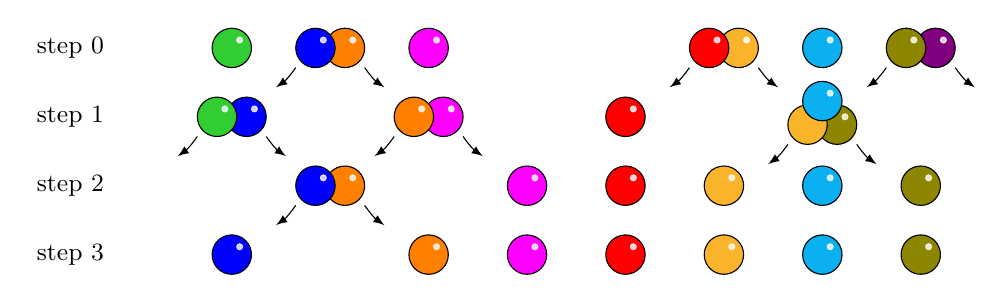
\begin{tikzpicture}[scale=0.25]
\node[anchor=east] at (-6, 0) {\small step 0};
\draw[fill=LimeGreen] (0, 0) ellipse (1 and 1);
\draw[fill=white,draw=white,opacity=0.8] (0+0.4, 0+0.4) ellipse (0.15 and 0.15);
\draw[fill=orange] (5.75, 0) ellipse (1 and 1);
\draw[fill=white,draw=white,opacity=0.8] (5.75+0.4, 0+0.4) ellipse (0.15 and 0.15);
\draw[fill=blue] (4.25, 0) ellipse (1 and 1);
\draw[fill=white,draw=white,opacity=0.8] (4.25+0.4, 0+0.4) ellipse (0.15 and 0.15);
\draw [->,>=latex] (3.25,-1) to[out=-125,in=35] (2.25,-2.0);
\draw [->,>=latex] (6.75,-1) to[out=-55,in=145] (7.75,-2.0);
\draw[fill=Magenta] (10, 0) ellipse (1 and 1);
\draw[fill=white,draw=white,opacity=0.8] (10+0.4, 0+0.4) ellipse (0.15 and 0.15);
\draw[fill=Dandelion] (25.75, 0) ellipse (1 and 1);
\draw[fill=white,draw=white,opacity=0.8] (25.75+0.4, 0+0.4) ellipse (0.15 and 0.15);
\draw[fill=red] (24.25, 0) ellipse (1 and 1);
\draw[fill=white,draw=white,opacity=0.8] (24.25+0.4, 0+0.4) ellipse (0.15 and 0.15);
\draw [->,>=latex] (23.25,-1) to[out=-125,in=35] (22.25,-2.0);
\draw [->,>=latex] (26.75,-1) to[out=-55,in=145] (27.75,-2.0);
\draw[fill=ProcessBlue] (30, 0) ellipse (1 and 1);
\draw[fill=white,draw=white,opacity=0.8] (30+0.4, 0+0.4) ellipse (0.15 and 0.15);
\draw[fill=violet] (35.75, 0) ellipse (1 and 1);
\draw[fill=white,draw=white,opacity=0.8] (35.75+0.4, 0+0.4) ellipse (0.15 and 0.15);
\draw[fill=olive] (34.25, 0) ellipse (1 and 1);
\draw[fill=white,draw=white,opacity=0.8] (34.25+0.4, 0+0.4) ellipse (0.15 and 0.15);
\draw [->,>=latex] (33.25,-1) to[out=-125,in=35] (32.25,-2.0);
\draw [->,>=latex] (36.75,-1) to[out=-55,in=145] (37.75,-2.0);
\node[anchor=east] at (-6, -3.5) {\small step 1};
\draw[fill=blue] (0.75, -3.5) ellipse (1 and 1);
\draw[fill=white,draw=white,opacity=0.8] (0.75+0.4, -3.5+0.4) ellipse (0.15 and 0.15);
\draw[fill=LimeGreen] (-0.75, -3.5) ellipse (1 and 1);
\draw[fill=white,draw=white,opacity=0.8] (-0.75+0.4, -3.5+0.4) ellipse (0.15 and 0.15);
\draw [->,>=latex] (-1.75,-4.5) to[out=-125,in=35] (-2.75,-5.5);
\draw [->,>=latex] (1.75,-4.5) to[out=-55,in=145] (2.75,-5.5);
\draw[fill=Magenta] (10.75, -3.5) ellipse (1 and 1);
\draw[fill=white,draw=white,opacity=0.8] (10.75+0.4, -3.5+0.4) ellipse (0.15 and 0.15);
\draw[fill=orange] (9.25, -3.5) ellipse (1 and 1);
\draw[fill=white,draw=white,opacity=0.8] (9.25+0.4, -3.5+0.4) ellipse (0.15 and 0.15);
\draw [->,>=latex] (8.25,-4.5) to[out=-125,in=35] (7.25,-5.5);
\draw [->,>=latex] (11.75,-4.5) to[out=-55,in=145] (12.75,-5.5);
\draw[fill=red] (20, -3.5) ellipse (1 and 1);
\draw[fill=white,draw=white,opacity=0.8] (20+0.4, -3.5+0.4) ellipse (0.15 and 0.15);
\draw[fill=olive] (30.75, -3.9) ellipse (1 and 1);
\draw[fill=white,draw=white,opacity=0.8] (30.75+0.4, -3.9+0.4) ellipse (0.15 and 0.15);
\draw[fill=Dandelion] (29.25, -3.9) ellipse (1 and 1);
\draw[fill=white,draw=white,opacity=0.8] (29.25+0.4, -3.9+0.4) ellipse (0.15 and 0.15);
\draw[fill=ProcessBlue] (30.0, -2.7) ellipse (1 and 1);
\draw[fill=white,draw=white,opacity=0.8] (30.0+0.4, -2.7+0.4) ellipse (0.15 and 0.15);
\draw [->,>=latex] (28.25,-4.9) to[out=-125,in=35] (27.25,-5.9);
\draw [->,>=latex] (31.75,-4.9) to[out=-55,in=145] (32.75,-5.9);
\node[anchor=east] at (-6, -7.0) {\small step 2};
\draw[fill=orange] (5.75, -7.0) ellipse (1 and 1);
\draw[fill=white,draw=white,opacity=0.8] (5.75+0.4, -7.0+0.4) ellipse (0.15 and 0.15);
\draw[fill=blue] (4.25, -7.0) ellipse (1 and 1);
\draw[fill=white,draw=white,opacity=0.8] (4.25+0.4, -7.0+0.4) ellipse (0.15 and 0.15);
\draw [->,>=latex] (3.25,-8.0) to[out=-125,in=35] (2.25,-9.0);
\draw [->,>=latex] (6.75,-8.0) to[out=-55,in=145] (7.75,-9.0);
\draw[fill=Magenta] (15, -7.0) ellipse (1 and 1);
\draw[fill=white,draw=white,opacity=0.8] (15+0.4, -7.0+0.4) ellipse (0.15 and 0.15);
\draw[fill=red] (20, -7.0) ellipse (1 and 1);
\draw[fill=white,draw=white,opacity=0.8] (20+0.4, -7.0+0.4) ellipse (0.15 and 0.15);
\draw[fill=Dandelion] (25, -7.0) ellipse (1 and 1);
\draw[fill=white,draw=white,opacity=0.8] (25+0.4, -7.0+0.4) ellipse (0.15 and 0.15);
\draw[fill=ProcessBlue] (30, -7.0) ellipse (1 and 1);
\draw[fill=white,draw=white,opacity=0.8] (30+0.4, -7.0+0.4) ellipse (0.15 and 0.15);
\draw[fill=olive] (35, -7.0) ellipse (1 and 1);
\draw[fill=white,draw=white,opacity=0.8] (35+0.4, -7.0+0.4) ellipse (0.15 and 0.15);
\node[anchor=east] at (-6, -10.5) {\small step 3};
\draw[fill=blue] (0, -10.5) ellipse (1 and 1);
\draw[fill=white,draw=white,opacity=0.8] (0+0.4, -10.5+0.4) ellipse (0.15 and 0.15);
\draw[fill=orange] (10, -10.5) ellipse (1 and 1);
\draw[fill=white,draw=white,opacity=0.8] (10+0.4, -10.5+0.4) ellipse (0.15 and 0.15);
\draw[fill=Magenta] (15, -10.5) ellipse (1 and 1);
\draw[fill=white,draw=white,opacity=0.8] (15+0.4, -10.5+0.4) ellipse (0.15 and 0.15);
\draw[fill=red] (20, -10.5) ellipse (1 and 1);
\draw[fill=white,draw=white,opacity=0.8] (20+0.4, -10.5+0.4) ellipse (0.15 and 0.15);
\draw[fill=Dandelion] (25, -10.5) ellipse (1 and 1);
\draw[fill=white,draw=white,opacity=0.8] (25+0.4, -10.5+0.4) ellipse (0.15 and 0.15);
\draw[fill=ProcessBlue] (30, -10.5) ellipse (1 and 1);
\draw[fill=white,draw=white,opacity=0.8] (30+0.4, -10.5+0.4) ellipse (0.15 and 0.15);
\draw[fill=olive] (35, -10.5) ellipse (1 and 1);
\draw[fill=white,draw=white,opacity=0.8] (35+0.4, -10.5+0.4) ellipse (0.15 and 0.15);
\end{tikzpicture}
\end{document}
